\documentclass[10pt
%usepdftitle=false,
% 	handout,
% 	notes,
% 	fleqn,
hyperref={
    pdfauthor={Hong Quan Ba Nguyen},
    pdftitle={Optimal Shape Design of Air Ducts in Combustion Engines: Design a General Framework},
    pdfsubject={Talk},
    pdfcreator={LaTeX},
}
]{beamer}

% use the beamerROMSOC theme
\mode<presentation>{\usetheme{romsoc}}
\beamertemplatenavigationsymbolsempty


% used packages
\usepackage[T1]{fontenc}
\usepackage[utf8]{vietnam}
\usepackage[utf8]{inputenc}
\usepackage{amsmath,amssymb,amsthm,mathtools}
\usepackage[english]{babel}
\usepackage{caption}
\usepackage{subcaption}

% used packages (for this presentation!)
%\usepackage{url}
%\newcommand{\at}{\makeatletter @\makeatother}


% ----------- title ------------------------------------------
% DON'T FORGET TO FILL IN YOUR INFORMATION IN DOCUMENTCLASS ON TOP
\title[Optimal Shape Design of Air Ducts]{Optimal Shape Design of Air Ducts in Combustion Engines}
\subtitle{Design a General Shape Optimization Framework}
\author[Name1 \and Name2]{Michael Hinterm\"uller \and Hồng Quản Bá Nguyễn}
\jointwork{Joint work with Karl Knall}
\institute[WIAS Berlin]{Weierstrass Institute for Applied Analysis {\small\&} Stochastics (WIAS Berlin)}
\date[Berlin, \today]{Berlin, \today}

% insert logos
%\insertLogoMatheon
%\insertLogoTUB
\insertLogoWIAS
\insertLogoHUB
%\insertLogoMathLab
%\insertLogoSISSA
%\insertLogoITMATI
%\insertLogoMOX
%\insertLogoPoliMi
%\insertLogoUHB
%\insertLogoINRIA
%\insertLogoBUW
%\insertLogoSTM
%\insertLogoMathConsult
%\insertLogoUSC
%\insertLogoDanieli
\insertLogoMathTec
%\insertLogoFAU   % not available yet



% set information on every page
\newcommand{\footinformationtext}{ROMSOC}	% Change here as required
\newcommand{\footinformationauthor}{}	% Change here as required

\footinformation{
    \vspace{0.7\baselineskip}
    \textcolor{romsocblue}{\rule[0.25\baselineskip]{0.97\textwidth}{0.6pt}} \par
    {\begin{minipage}[t]{0.4\textwidth}
            \settowidth{\fiwidth}{\footinformationtext}
            \vspace{-1.0\baselineskip}
            \hspace{0.66\baselineskip} 
            \footinformationtext \par
    \end{minipage}}\hfill
    {\begin{minipage}[t]{0.35\textwidth}
            \settowidth{\faiwidth}{\footinformationauthor}
            \vspace{-1.0\baselineskip}
            \footinformationauthor \par
    \end{minipage}}\hfill
}


\newlength{\pagenumberwidtha} %Deklaration
\newlength{\titlewidth} %Deklaration
\newlength{\logowidth} %Deklaration
\newlength{\fiwidth} %Deklaration
\newlength{\faiwidth} %Deklaration


% ----------- document --------------------------------------------------------
\begin{document}
\maketitle
\AtBeginSection[]{   %set the overview slide before every section
    \begin{frame}%[noframenumbering]
        \frametitle{Outline}
        %\begin{tocbox}{}
        \tableofcontents[current]
        %\end{tocbox}
    \end{frame}
}

% ----------- frames ----------------------------------------------------------
\section{Targets}

\begin{frame}{Combustion engines}
    \vspace{5mm}   
    \begin{figure}
        \begin{subfigure}{.49\textwidth}
            \centering
            % include first image
            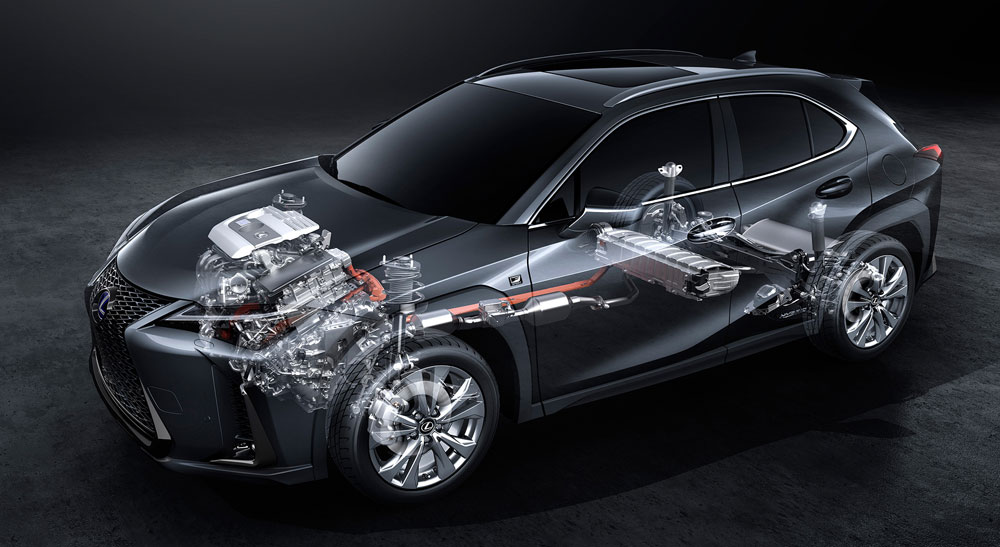
\includegraphics[width=.7\linewidth]{Combustion_Engine_in_Car}  
            \caption{\href{https://lexusenthusiast.com/2018/04/24/internal-combustion-engines-remain-priority-at-toyota/}{Toyota car}.}
            \label{fig:sub-first}
        \end{subfigure}        
        \begin{subfigure}{.49\textwidth}
            \centering
            % include fourth image
            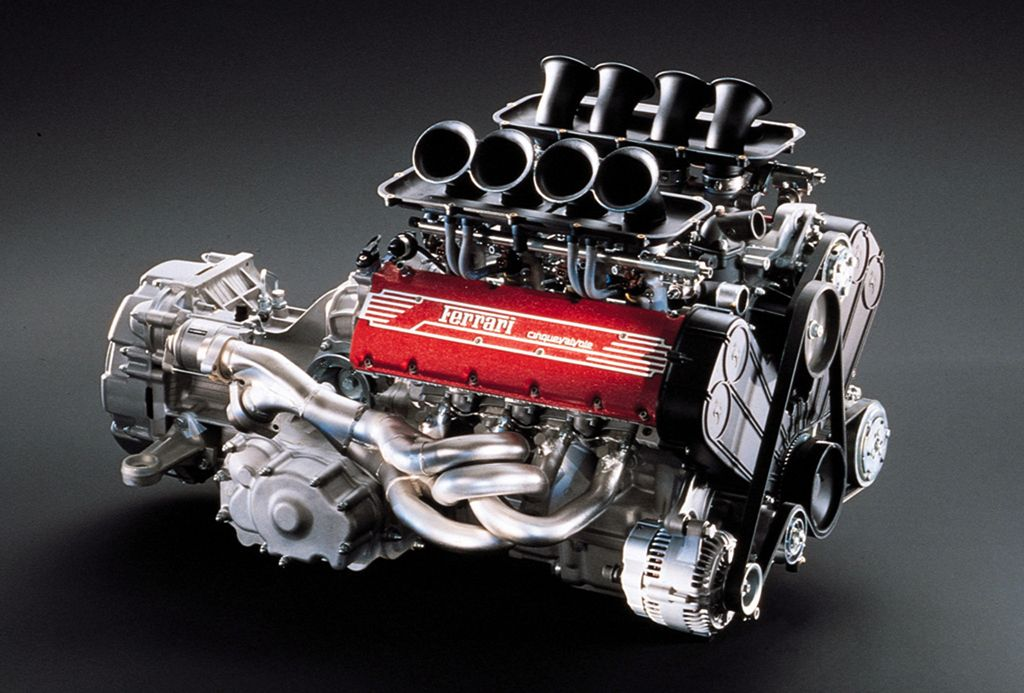
\includegraphics[width=.7\linewidth]{Ferrari_355_Engine}  
            \caption{Ferrari combustion engine.}
            \label{fig:sub-fourth}
        \end{subfigure}    
        \begin{subfigure}{.49\textwidth}
            \centering
            % include third image
            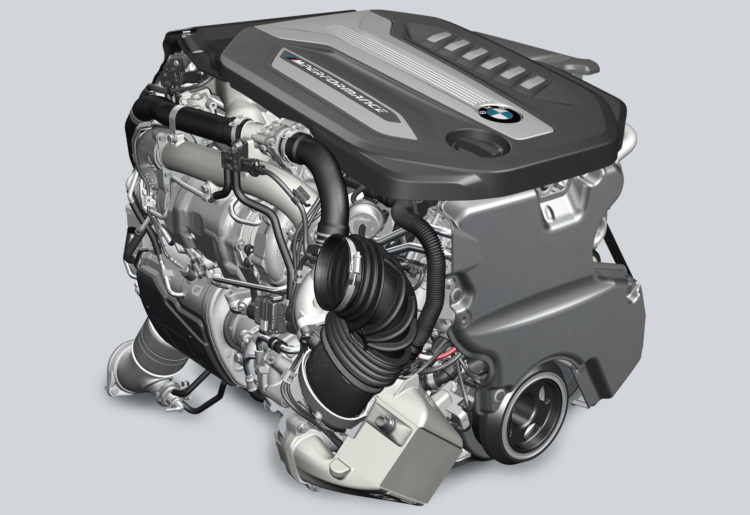
\includegraphics[width=.7\linewidth]{BMW_Combustion_Engine}  
            \caption{\href{https://www.bmwblog.com/2019/06/27/bmw-sees-internal-combustion-engines-still-going-for-a-couple-decades/}{BMW combustion engine}.}
            \label{fig:sub-third}
        \end{subfigure}
        \begin{subfigure}{.49\textwidth}
            \centering
            % include second image
            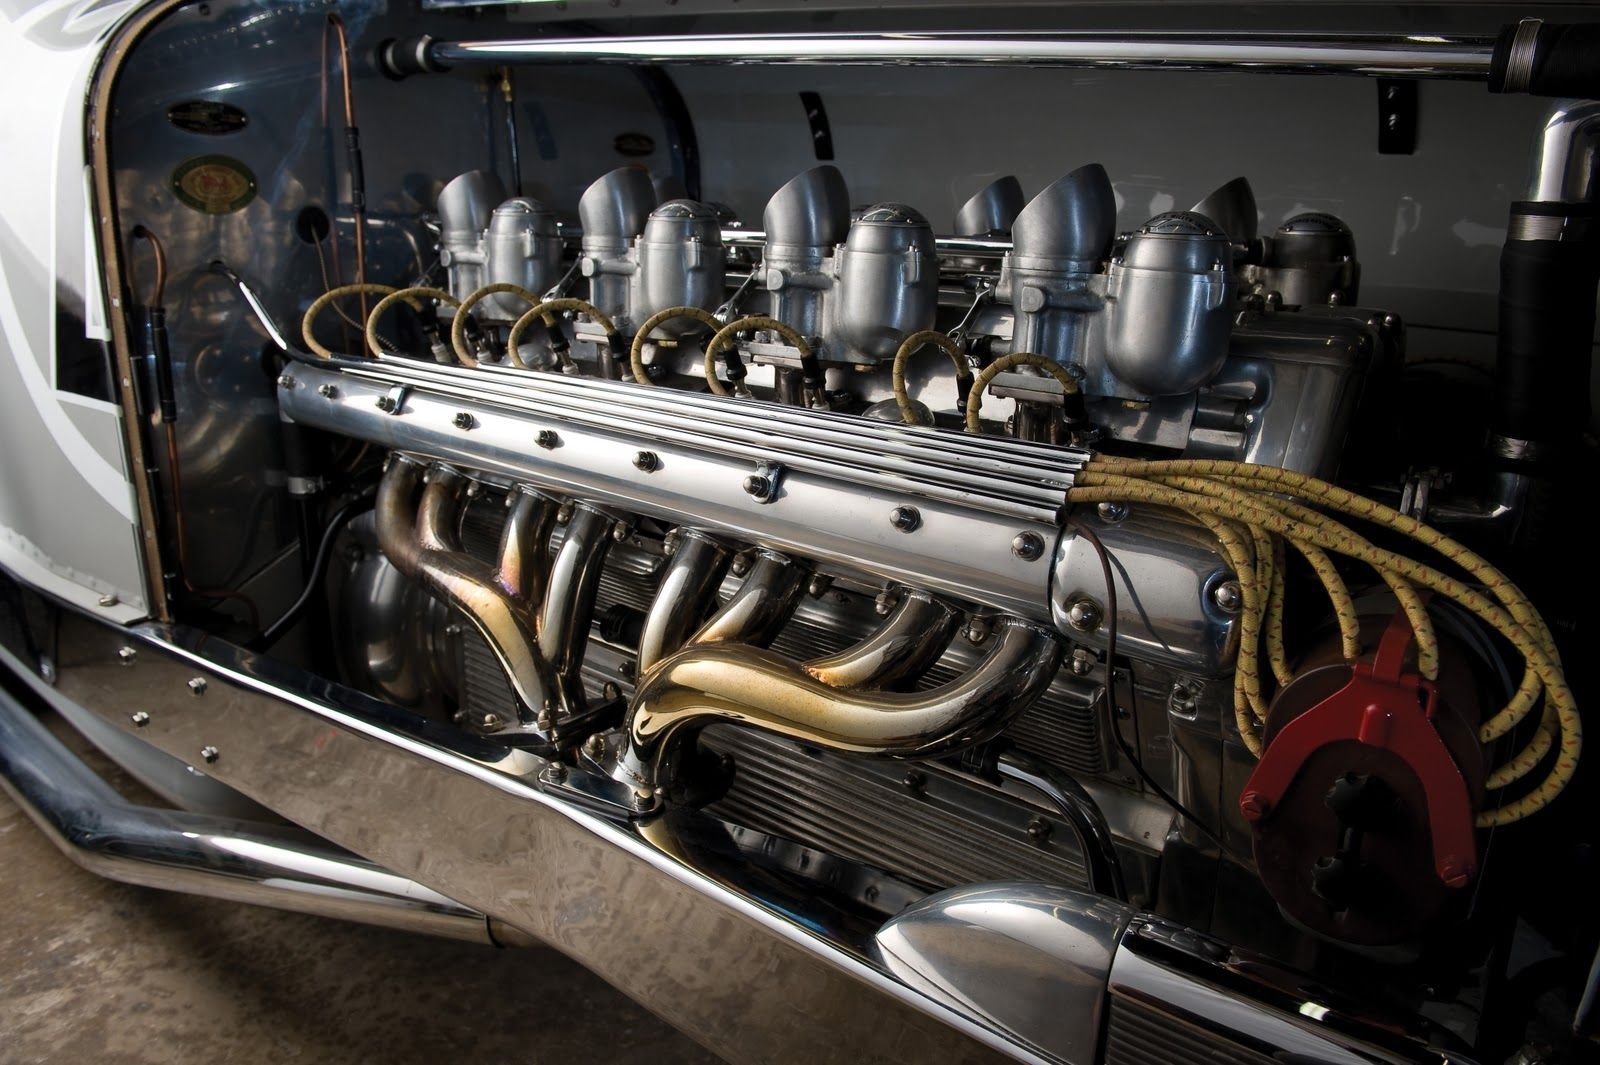
\includegraphics[width=.7\linewidth]{Combustion_Engines_1}  
            \caption{\href{https://www.pinterest.es/pin/816136763692046539/}{A beautiful combustion engine.}}
            \label{fig:sub-second}
        \end{subfigure}
    \end{figure}
\end{frame}

\begin{frame}{Air duct models}
    \begin{itemize}
        \item A schematic 1-inlet-1-outlet duct geometry {\small\&} its boundary:
        \begin{figure}
            \centering
            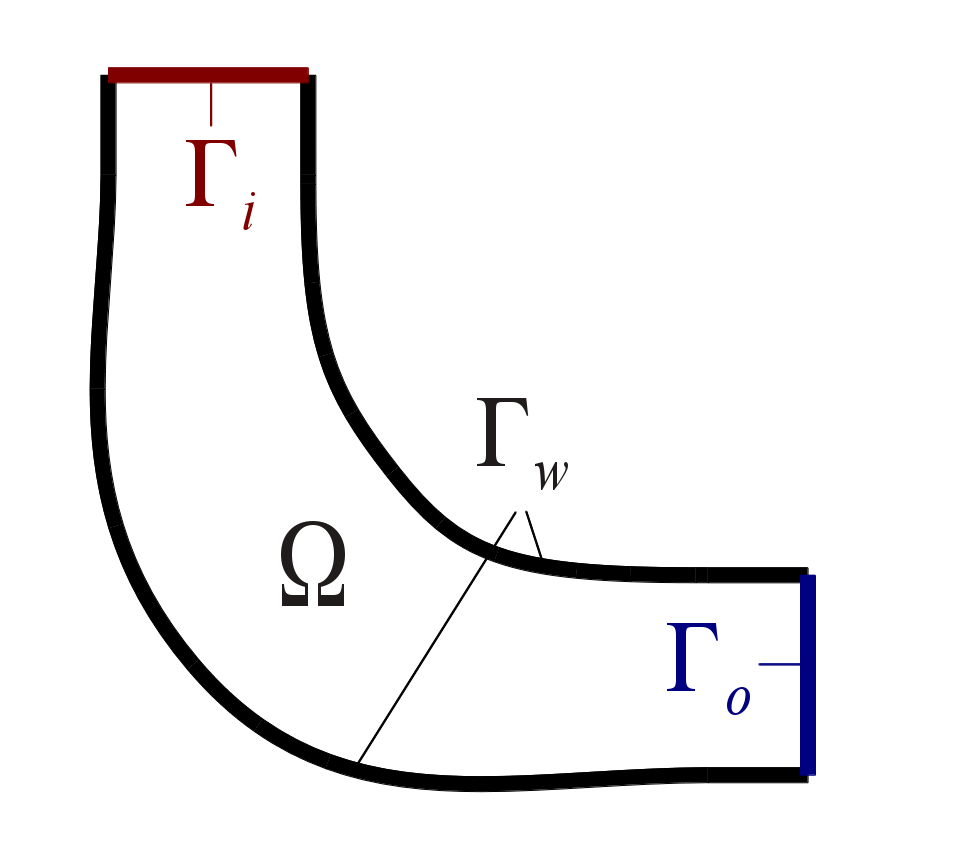
\includegraphics[scale=0.55]{Geometry_Simple_Sketch}
            \caption{A simple sketch of a 1-inlet-1-outlet air duct.}
        \end{figure}
        \item Air ducts with multiple inlets {\small\&}\texttt{/}or outlets $\to$ later.
        \item \textbf{Target.} \fbox{Optimize the shape of air ducts.}
    \end{itemize}
\end{frame}

\begin{frame}{Instationary incompressible viscous Navier-Stokes equations}
    A BVP for the instationary incompressible viscous NSEs with \textit{mixed boundary conditions}:
    \begin{equation}
        \label{instationary incompressible viscous NSEs}
        \tag{iNS}
        \left\{\begin{split}
            \textbf{u}_t - \nu\Delta\textbf{u} + (\textbf{u}\cdot\nabla)\textbf{u} + \nabla p &= \textbf{f} &&\mbox{ in } (0,T)\times\Omega,\\
            \nabla\cdot\textbf{u} &= 0 &&\mbox{ in } (0,T)\times\Omega,\\
            \textbf{u}(0,\cdot) &= \textbf{u}_0 &&\mbox{ in } \Omega,\\
            \textbf{u} &= \textbf{f}_{\rm in} &&\mbox{ on } [0,T]\times\Gamma_{\rm in},\\
            \textbf{u} &= \textbf{0} &&\mbox{ on } [0,T]\times\Gamma_{\rm wall},\\
            -\nu\partial_{\textbf{n}}\textbf{u} + p\textbf{n} &= \textbf{0} &&\mbox{ on } [0,T]\times\Gamma_{\rm out},
        \end{split}\right.
    \end{equation}
    where \begin{itemize}
        \item $\textbf{u}:[0,T]\times\Omega\to\mathbb{R}^N$: velocity, $p:[0,T]\times\Omega\to\mathbb{R}$: pressure;
        \item $\nu > 0$: kinematic viscosity, $\textbf{f}$: source term, $\textbf{u}_0$: initial velocity, $\textbf{f}_{\rm in}$: inflow profile at $\Gamma_{\rm in}$.
    \end{itemize}
\end{frame}

\begin{frame}{Cost\texttt{/}Shape functionals}
    \begin{itemize}
        \item \textbf{Flow uniformity at the outlet.}
        \begin{itemize}
            \item An important design criterion of \textit{automotive air ducts}.
            \item Efficiently distribute fresh air inside cars\texttt{/}engines.
        \end{itemize}
        \begin{align}
            \label{cost functional: outflow uniformity}
            \tag{$J_1$}
            J_1(\textbf{u},\Omega)\coloneqq\frac{1}{2}\int_0^T\int_{\Gamma_{\textrm{out}}} \left(\textbf{u}\cdot\textbf{n} - \overline{u}\right)^2\textrm{d}\Gamma\textrm{d}t,
        \end{align}
        with a desired value $\overline{u}$, e.g.:
        \begin{align*}
            \overline{u}\coloneqq -\frac{1}{TH_{N-1}(\Gamma_{\textrm{out}})}\int_0^T\int_{\Gamma_{\textrm{in}}} \textbf{f}_{\textrm{in}}\cdot\textbf{n}\textrm{d}\Gamma\textrm{d}t,
        \end{align*}
        where $H_{N-1}(\cdot)$: $(N - 1)$-dimensional Hausdorff measure.
    \end{itemize}
\end{frame}

\begin{frame}{Cost\texttt{/}Shape functionals}
    \begin{itemize}
        \item \textbf{Energy dissipation.}
        \begin{itemize}
            \item Minimize the power dissipated by air ducts\texttt{/}any fluid dynamics devices.
            \item Compute the dissipated power as the net inward flux of energy through the boundary:
        \end{itemize}
        \begin{align}
            \label{cost functional: energy dissipation}
            \tag{$J_2$}
            J_2(\textbf{u},p,\Omega)\coloneqq -\int_0^T\int_\Gamma \left(p + \frac{1}{2}|\textbf{u}|^2\right)\textbf{u}\cdot\textbf{n}\textrm{d}\Gamma\textrm{d}t.
        \end{align}
    \end{itemize}
    \textbf{Regularity of \eqref{instationary incompressible viscous NSEs}.} $(\textbf{u},p)\in W^{1,2}(\Omega;\mathbb{R}^N)\times L^2(\Omega)$ usually \cite{MR2009}.
    
    Consider an approximation of $J_2$, with thickness $\delta > 0$:
    \begin{align}
        J_2^\delta(\textbf{u},p,\Omega)\coloneqq&\, -\frac{H_{N-1}(\Gamma_{\textrm{in}})}{\operatorname{m}_N(\Gamma_{\textrm{in}}^\delta)}\int_0^T\int_{\Gamma_{\textrm{in}}^\delta} \left(p + \frac{1}{2}|\textbf{u}|^2\right)\textbf{u}\cdot\textbf{n}\textrm{d}\textbf{x}\textrm{d}t\nonumber\\
        & - \frac{H_{N-1}(\Gamma_{\textrm{out}})}{\operatorname{m}_N(\Gamma_{\textrm{out}}^\delta)}\int_0^T\int_{\Gamma_{\textrm{out}}^\delta} \left(p + \frac{1}{2}|\textbf{u}|^2\right)\textbf{u}\cdot\textbf{n}\textrm{d}\textbf{x}\textrm{d}t.\label{cost functional: approximated energy dissipation}
        \tag{$J_2^\delta$}
    \end{align}
\end{frame}

\begin{frame}{Cost\texttt{/}Shape functionals}
    \begin{align*}
        J_2^\delta(\textbf{u},p,\Omega) =& \int_0^T\int_\Omega k_\delta(\textbf{x})\left(p + \frac{1}{2}|\textbf{u}|^2\right)\textbf{u}\cdot\textbf{n}\textrm{d}\textbf{x}\textrm{d}t,
    \end{align*}
    where $\operatorname{m}_N$ denotes the $N$-dimensional Lebesgue measure {\small\&}
    \begin{align*}
        k_\delta(\textbf{x})\coloneqq -\frac{H_{N-1}(\Gamma_{\textrm{in}})}{\operatorname{m}_N(\Gamma_{\textrm{in}}^\delta)}\chi_{\Gamma_{\textrm{in}}^\delta}(\textbf{x}) - \frac{H_{N-1}(\Gamma_{\textrm{out}})}{\operatorname{m}_N(\Gamma_{\textrm{out}}^\delta)}\chi_{\Gamma_{\textrm{out}}^\delta}(\textbf{x}),\ \forall\textbf{x}\in\Omega.
    \end{align*}
    \begin{figure}[h]
        \centering
        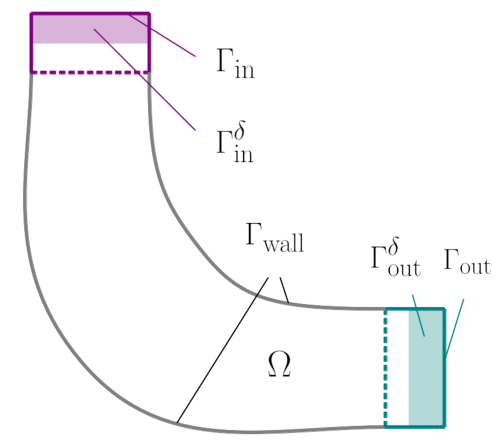
\includegraphics[width=0.35\textwidth]{geometry_delta}
        \caption{The duct geometry with $\delta$-approximated inlet $\Gamma_{\textrm{in}}^\delta$ {\small\&} outlet $\Gamma_{\textrm{out}}^\delta$.}
        \label{fig:geometry cutoff inlet outlet}
    \end{figure}
\end{frame}

\begin{frame}{Mixed cost functional {\small\&} a shape optimization problem}
    A mixed cost functional with a weighting parameter $\gamma\in[0,1]$:
    \begin{align}
        \label{mixed cost functional}
        \tag{$J_{12}^{\delta,\gamma}$}
        J_{12}^{\delta,\gamma}(\textbf{u},p,\Omega)\coloneqq&\, (1 - \gamma)J_1(\textbf{u},\Omega) + \gamma J_2^\delta(\textbf{u},p,\Omega)\\
        =&\, \frac{1 - \gamma}{2}\int_0^T\int_{\Gamma_{\textrm{out}}} \left(\textbf{u}\cdot\textbf{n} - \overline{u}\right)^2\textrm{d}\Gamma\textrm{d}t\nonumber\\
        &+ \int_0^T\int_\Omega \gamma k_\delta(\textbf{x})\left(p + \frac{1}{2}|\textbf{u}|^2\right)\textbf{u}\cdot\textbf{n}\textrm{d}\textbf{x}\textrm{d}t.\nonumber
    \end{align}
    A PDEs-constrained shape optimization problem (SOP):
    \begin{align}
        \label{shape optimization problem}
        \tag{sop}
        \boxed{\min_{\Omega\in\mathcal{O}_{\textrm{ad}}} J_{12}^{\delta,\gamma}(\textbf{u},p,\Omega) \mbox{ s.t. } (\textbf{u},p) \mbox{ solves \eqref{instationary incompressible viscous NSEs}}.}
    \end{align}    
\end{frame}

\begin{frame}{Targets}
    \begin{itemize}
        \item Topology Optimization [later] {\small\&} Shape Optimization for BVPs of
        \begin{itemize}
            \item Stationary Navier-Stokes equations
            \item Instationary Navier-Stokes equations
            \item Large Eddy Simulation (LES), e.g., Smagorinsky turbulence model
            \item Reynolds-averaged Navier-Stokes (RANS) equations, e.g., $k$-$\epsilon$ turbulence model \cite{MP1994}
        \end{itemize}
        in 2D {\small\&} 3D with mixed boundary conditions.
        \item Develop FEM\texttt{/}FVM-based (e.g., FEniCS\texttt{/}OpenFOAM-based) software to implement the continuous adjoint approach.
    \end{itemize}
\end{frame}

\section{A framework for PDEs-constrained shape optimization problems}

\begin{frame}{A general model {\small\&} cost\texttt{/}shape functional}
    \begin{itemize}
        \item A general stationary PDEs for velocity $\textbf{u}$ {\small\&} pressure $p$:
        \begin{equation}
            \label{general stationary fluid dynamics PDEs}
            \tag{gfld}
            \boxed{\left\{\begin{split}
                \textbf{P}(\textbf{x},\textbf{u},\nabla\textbf{u},\Delta\textbf{u},p,\nabla p) &= \textbf{f}(\textbf{x},\textbf{u},\nabla\textbf{u},p) &&\mbox{ in } \Omega,\\
                -\nabla\cdot\textbf{u} &= f_{\rm div}(\textbf{x},\textbf{u},\nabla\textbf{u},p) &&\mbox{ in } \Omega,\\
                \textbf{Q}(\textbf{x},\textbf{u},\nabla\textbf{u},p,\textbf{n},\textbf{t}) &= \textbf{f}_{\rm bc}(\textbf{x}) &&\mbox{ on } \Gamma,
            \end{split}\right.}
        \end{equation}
        where $\textbf{P}(\cdot,\ldots,\cdot)$ denotes the main PDEs (e.g., momentum conservation equations), $\textbf{Q}(\cdot,\ldots,\cdot)$ denotes the boundary conditions (BCs).
        \item A general cost functional for \eqref{general stationary fluid dynamics PDEs}:
        \begin{align}
            \label{cost functional for general stationary fluid dynamics PDEs}
            \tag{cost-gfld}
            \boxed{J(\textbf{u},p,\Omega)\coloneqq\int_\Omega J_\Omega(\textbf{x},\textbf{u},\nabla\textbf{u},p){\rm d}\textbf{x} + \int_\Gamma J_\Gamma(\textbf{x},\textbf{u},\nabla\textbf{u},p,\textbf{n},\textbf{t}){\rm d}\Gamma.}
        \end{align}
    \end{itemize}
\end{frame}

\begin{frame}{Lagrangians}
    To derive the adjoint equations for \eqref{general stationary fluid dynamics PDEs}, introduce:
    \begin{itemize}
        \item \textbf{Standard Lagrangian}:
        \begin{align}
            &L(\textbf{u},p,\Omega,\textbf{v},q)\nonumber\\
            &\coloneqq J(\textbf{u},p,\Omega) + \int_\Omega -\left(\textbf{P}(\textbf{x},\textbf{u},\nabla\textbf{u},\Delta\textbf{u},p,\nabla p) - \textbf{f}(\textbf{x},\textbf{u},\nabla\textbf{u},p)\right)\cdot\textbf{v}\nonumber\\
            &\hspace{3.05cm}+ q\left(\nabla\cdot\textbf{u} + f_{\rm div}(\textbf{x},\textbf{u},\nabla\textbf{u},p)\right){\rm d}\textbf{x}.\label{Lagrangian for general stationary fluid dynamics PDEs}
            \tag{$L$-gfld}
        \end{align}
        \item \textbf{Extended Lagrangian}:
        \begin{align}            
            &\mathcal{L}(\textbf{u},p,\Omega,\textbf{v},q,\textbf{v}_{\rm bc})\nonumber\\
            &\coloneqq L(\textbf{u},p,\Omega,\textbf{v},q) - \int_\Gamma \left(\textbf{Q}(\textbf{x},\textbf{u},\nabla\textbf{u},p,\textbf{n},\textbf{t}) - \textbf{f}_{\rm bc}(\textbf{x})\right)\cdot\textbf{v}_{\rm bc}{\rm d}\Gamma.\label{extended Lagrangian for general stationary fluid dynamics PDEs}
            \tag{$\mathcal{L}$-gfld}
        \end{align}
    \end{itemize}
    where $\textbf{v}$, $q$, $\textbf{v}_{\rm bc}$ are Lagrange multipliers.
\end{frame}

\begin{frame}{Shape optimization problems (SOPs)}
    Consider 3 different SOPs for \eqref{cost functional for general stationary fluid dynamics PDEs}, \eqref{Lagrangian for general stationary fluid dynamics PDEs}, {\small\&} \eqref{extended Lagrangian for general stationary fluid dynamics PDEs}, resp.:
    \begin{itemize}
        \item Treat the whole of \eqref{general stationary fluid dynamics PDEs} as equality constraints:
        \begin{align}
            &\boxed{\min_{\Omega\in\mathcal{O}_{\rm ad}} J(\textbf{u},p,\Omega) \mbox{ s.t. } (\textbf{u},p) \mbox{ solves \eqref{general stationary fluid dynamics PDEs}},}\label{SOP for cost functional for general stationary fluid dynamics PDEs}\tag{sop-$J$-gfld}
        \end{align}
        \item Penalize the 1st 2 equations of \eqref{general stationary fluid dynamics PDEs} but keep the BCs as an equality constraint:
        \begin{align}
            \boxed{\min_{\Omega\in\mathcal{O}_{\rm ad}} L(\textbf{u},p,\Omega,\textbf{v},q) \mbox{ s.t. } (\textbf{u},p) \mbox{ s.t. } \textbf{Q}(\textbf{x},\textbf{u},\nabla\textbf{u},p,\textbf{n},\textbf{t}) = \textbf{f}_{\rm bc}(\textbf{x}) \mbox{ on } \Gamma,}\label{SOP for Lagrangian for general stationary fluid dynamics PDEs}\tag{sop-$L$-gfld}
        \end{align}
        \item Penalize all of \eqref{general stationary fluid dynamics PDEs}:
        \begin{align}
            \boxed{\min_{\Omega\in\mathcal{O}_{\rm ad}} \mathcal{L}(\textbf{u},p,\Omega,\textbf{v},q,\textbf{v}_{\rm bc}) \mbox{ with } (\textbf{u},p) \mbox{ unconstrained}.}\label{SOP for extended Lagrangian for general stationary fluid dynamics PDEs}\tag{sop-$\mathcal{L}$-gfld}
        \end{align}
    \end{itemize}
\end{frame}

\begin{frame}{Mixed Lagrangian {\small\&} mixed SOP}
    \begin{itemize}
        \item \textbf{Question.} \textit{Use standard\texttt{/}extended Lagrangian to derive adjoint PDEs?}
        \item Consider a ``mixed Lagrangian'' with a ``switch'' $\delta_{\mathcal{L}}\in\{0,1\}$:
        \begin{align}
            \label{mixed Lagrangian for general stationary fluid dynamics PDEs}
            \tag{$\mathcal{L}$-gfld}
            L_{\mathcal{L}}(\textbf{u},p,\Omega,\textbf{v},q,\textbf{v}_{\rm bc})\coloneqq L - \delta_{\mathcal{L}}\int_\Gamma \left(\textbf{Q} - \textbf{f}_{\rm bc}\right)\cdot\textbf{v}_{\rm bc}{\rm d}\Gamma.
        \end{align}
        Hence,
        \begin{equation*}
            L_{\mathcal{L}}(\textbf{u},p,\Omega,\textbf{v},q,\textbf{v}_{\rm bc}) = \left\{\begin{split}
                &L(\textbf{u},p,\Omega,\textbf{v},q) &&\mbox{ if } \delta_{\mathcal{L}} = 0,\\
                &\mathcal{L}(\textbf{u},p,\Omega,\textbf{v},q,\textbf{v}_{\rm bc}) &&\mbox{ if } \delta_{\mathcal{L}} = 1.
            \end{split}\right.
        \end{equation*}
        \item 4th SOP (a combination of 2nd {\small\&} 3rd SOPs):
        \begin{equation}
            \label{SOP for mixed Lagrangian for general stationary fluid dynamics PDEs}\tag{sop-$L_{\mathcal{L}}$-gfld}
            \boxed{\min_{\Omega\in\mathcal{O}_{\rm ad}} L_{\mathcal{L}}(\textbf{u},p,\Omega,\textbf{v},q,\textbf{v}_{\rm bc})\ \left\{\begin{split}
                &\mbox{s.t. } (\textbf{u},p) \mbox{ s.t. } \textbf{Q} = \textbf{f}_{\rm bc} \mbox{ on } \Gamma &&\mbox{ if } \delta_{\mathcal{L}} = 0,\\
                &\mbox{with } (\textbf{u},p) \mbox{ unconstrained} &&\mbox{ if } \delta_{\mathcal{L}} = 1.
            \end{split}\right.}
        \end{equation}
    \end{itemize}
\end{frame}

\begin{frame}{Derive adjoint PDEs}
    \begin{itemize}
        \item Formally, if $(\textbf{u}^\star,p^\star,\Omega^\star)$ is an optimal point, then
        \begin{align*}
            D_{(\textbf{u},p)}L_{\mathcal{L}}(\textbf{u}^\star,p^\star,\Omega^\star,\textbf{v},q,\textbf{v}_{\rm bc})(\tilde{\textbf{u}},\tilde{p}) = 0,\ \forall(\tilde{\textbf{u}},\tilde{p}).
        \end{align*}
        \item Choose the adjoint variables\texttt{/}Lagrange multipliers $(\textbf{v},q,\textbf{v}_{\rm bc})$ s.t.
        \begin{align*}
            \boxed{D_{\textbf{u}}L_{\mathcal{L}}(\textbf{u}^\star,p^\star,\Omega^\star,\textbf{v},q,\textbf{v}_{\rm bc})\tilde{\textbf{u}} + D_pL_{\mathcal{L}}(\textbf{u}^\star,p^\star,\Omega^\star,\textbf{v},q,\textbf{v}_{\rm bc})\tilde{p} = 0,}
        \end{align*}
        for all $(\textbf{u},p,\Omega,\tilde{\textbf{u}},\tilde{p})$, where $\tilde{\textbf{u}}$, $\tilde{p}$: variations of $\textbf{u}$, $p$, resp.
        \item Expand this explicitly, $\forall(\textbf{u},p,\Omega,\tilde{\textbf{u}},\tilde{p})$:
        \begin{align*}
            &\int_\Omega \left[F_\Omega^{\Delta\tilde{\textbf{u}}}(\cdot)\Delta\tilde{\textbf{u}} + F_\Omega^{\nabla\tilde{\textbf{u}}}(\cdot)\nabla\tilde{\textbf{u}} + F_\Omega^{\tilde{\textbf{u}}}(\cdot)\tilde{\textbf{u}} + F_\Omega^{\tilde{p}}(\cdot)\tilde{p} + F_\Omega^{\nabla\tilde{p}}(\cdot)\nabla\tilde{p}\right]\cdot\{\textbf{v},q\}{\rm d}\textbf{x}\\
            &+ D_{(\textbf{u},p)}J(\textbf{u},p,\Omega)(\tilde{\textbf{u}},\tilde{p}) + \delta_{\mathcal{L}}\int_\Gamma \left[F_\Gamma^{\nabla\tilde{\textbf{u}}}(\cdot)\nabla\tilde{\textbf{u}} + F_\Gamma^{\tilde{\textbf{u}}}(\cdot)\tilde{\textbf{u}} + F_\Gamma^{\tilde{p}}(\cdot)\tilde{p}\right]\cdot\textbf{v}_{\rm bc}{\rm d}\Gamma\\
            &= 0, \mbox{ where } (\cdot)|_\Omega = (\textbf{x},\textbf{u},\nabla\textbf{u},\Delta\textbf{u},p,\nabla p),\ (\cdot)|_\Gamma = (\textbf{x},\textbf{u},\nabla\textbf{u},p,\textbf{n},\textbf{t},\textbf{v}_{\rm bc}).
        \end{align*}
    \end{itemize}
\end{frame}

\begin{frame}{Derive adjoint of \eqref{general stationary fluid dynamics PDEs}: integrate by parts}
    \begin{itemize}
        \item Let $A:D(A)\subset E\to F$: an unbounded linear operator [Brezis2010]. Adjoint of $A$: the unbounded linear operator $A^\star:D(A^\star)\subset F^\star\to E^\star$ s.t.
        \begin{align*}
            \langle v,Au\rangle_{F^\star,F} = \langle A^\star v,u\rangle_{E^\star,E},\ \forall u\in D(A),\ \forall v\in D(A^\star).
        \end{align*}
        \item Analogously, rewrite the current equation:
        \begin{align*}
            &\left(1,A_{J_\Omega}(\tilde{\textbf{u}},\tilde{p})\right)_{L^2(\Omega)} + \left(1,A_{J_\Gamma}(\tilde{\textbf{u}},\tilde{p})\right)_{L^2(\Gamma)} + \left((\textbf{v},q), A_\Omega(\tilde{\textbf{u}},\tilde{p})\right)_{L^2(\Omega)}\\
            &\hspace{5mm}+ \delta_{\mathcal{L}}\left(\textbf{v}_{\rm bc},A_\Gamma(\tilde{\textbf{u}},\tilde{p})\right)_{L^2(\Gamma)} = 0,\ \forall(\textbf{u},p,\Omega,\tilde{\textbf{u}},\tilde{p}).
        \end{align*}
        \item \textbf{Goal.} Integrate by parts to obtain:
        \begin{align*}
            &\left(A_{J_\Omega}^\star 1,(\tilde{\textbf{u}},\tilde{p})\right)_{L^2(\Omega)} + \left(1,A_{J_\Gamma}(\tilde{\textbf{u}},\tilde{p})\right)_{L^2(\Gamma)} + \left(A_\Omega^\star(\textbf{v},q), (\tilde{\textbf{u}},\tilde{p})\right)_{L^2(\Omega)}\\
            &\hspace{5mm}+ \delta_{\mathcal{L}}\left(\textbf{v}_{\rm bc},A_\Gamma(\tilde{\textbf{u}},\tilde{p})\right)_{L^2(\Gamma)} = 0,\ \forall(\textbf{u},p,\Omega,\tilde{\textbf{u}},\tilde{p}).
        \end{align*}
    \item \textbf{Question.} \textit{Integrate by parts which terms?}
    \end{itemize}
\end{frame}

\begin{frame}{Derive adjoint of \eqref{general stationary fluid dynamics PDEs}: integrate by parts}
    \begin{itemize}
        \item Roughly speaking,
        \begin{align*}
            \int_\Omega F_\Omega\{\nabla\tilde{\textbf{u}},\Delta\tilde{\textbf{u}},\nabla\tilde{p}\}\cdot\{\textbf{v},q\}{\rm d}\textbf{x}\xrightarrow{\rm i.b.p.}&\int_\Omega \{\tilde{\textbf{u}},\tilde{p}\}\cdot F_\Omega^\star\{\nabla\textbf{v},\Delta\textbf{v},\nabla q\}{\rm d}\textbf{x}\\
            &+ \mbox{ by-products } \int_\Gamma \cdots{\rm d}\Gamma.
        \end{align*}
        \item Integrate by parts all the red terms:
        \begin{align*}
            &\int_\Omega \left[{\color{red}F_\Omega^{\Delta\tilde{\textbf{u}}}(\cdot)\Delta\tilde{\textbf{u}}} + {\color{red}F_\Omega^{\nabla\tilde{\textbf{u}}}(\cdot)\nabla\tilde{\textbf{u}}} + F_\Omega^{\tilde{\textbf{u}}}(\cdot)\tilde{\textbf{u}} + F_\Omega^{\tilde{p}}(\cdot)\tilde{p} + {\color{red}F_\Omega^{\nabla\tilde{p}}(\cdot)\nabla\tilde{p}}\right]{\color{red}\cdot\{\textbf{v},q\}}{\rm d}\textbf{x}\\
            &+ \int_\Omega {\color{red}D_{\nabla\textbf{u}}J_\Omega(\cdot)\nabla\tilde{\textbf{u}}}{\rm d}\textbf{x} + \mbox{ the rest of } D_{(\textbf{u},p)}J(\textbf{u},p,\Omega)\\
            &+ \delta_{\mathcal{L}}\int_\Gamma \left[F_\Gamma^{\nabla\tilde{\textbf{u}}}(\cdot)\nabla\tilde{\textbf{u}} + F_\Gamma^{\tilde{\textbf{u}}}(\cdot)\tilde{\textbf{u}} + F_\Gamma^{\tilde{p}}(\cdot)\tilde{p}\right]\cdot\textbf{v}_{\rm bc}{\rm d}\Gamma = 0.
        \end{align*}
    \end{itemize}
\end{frame}

\begin{frame}{Derive adjoint of \eqref{general stationary fluid dynamics PDEs} with extended Lagrangian \eqref{extended Lagrangian for general stationary fluid dynamics PDEs}}
    Assume $\delta_{\mathcal{L}} = 1$. Gather terms: $\forall(\textbf{u},p,\Omega,\tilde{\textbf{u}},\tilde{p})$,
    \begin{align*}
        \int_\Omega \textbf{F}_\Omega^{\tilde{\textbf{u}}}(\cdot)\cdot\tilde{\textbf{u}} + F_\Omega^{\tilde{p}}(\cdot)\tilde{p}{\rm d}\textbf{x} + \int_\Gamma \textbf{F}_\Gamma^{\tilde{\textbf{u}}}(\cdot)\cdot\tilde{\textbf{u}} + F_\Gamma^{\tilde{p}}(\cdot)\tilde{p} + F_\Gamma^{\nabla\tilde{\textbf{u}}}(\cdot,\nabla\tilde{\textbf{u}}){\rm d}\Gamma = 0,
    \end{align*}
    \begin{itemize}
        \item Choose $\tilde{\textbf{u}}|_{\overline{\Omega}} = \textbf{0}$, $\int_\Omega F_\Omega^{\tilde{p}}(\cdot)\tilde{p}{\rm d}\textbf{x} + \int_\Gamma F_\Gamma^{\tilde{p}}(\cdot)\tilde{p}{\rm d}\Gamma = 0$, $\forall(\textbf{u},p,\Omega,\tilde{p})$.
        \begin{itemize}
            \item Choose $\tilde{p}$ s.t. $\tilde{p}|_\Gamma = 0$, then $\int_\Omega F_\Omega^{\tilde{p}}(\cdot)\tilde{p}{\rm d}\textbf{x} = 0$ $\forall(\textbf{u},p,\Omega,\tilde{p})$ s.t. $\tilde{p}|_\Gamma = 0$, thus
            \begin{align*}
                \boxed{F_\Omega^{\tilde{p}}(\textbf{x},\textbf{u},\nabla\textbf{u},\Delta\textbf{u},p,\nabla p,\textbf{v},\nabla\textbf{v},q) = 0 \mbox{ in } \Omega.}
            \end{align*}
            \item Plug it back in, obtain $\int_\Gamma F_\Gamma^{\tilde{p}}(\cdot)\tilde{p}{\rm d}\Gamma = 0$, $\forall(\textbf{u},p,\Omega,\tilde{p})$, thus
            \begin{align*}
                \boxed{F_\Gamma^{\tilde{p}}(\cdot)(\textbf{x},\textbf{u},\nabla\textbf{u},\Delta\textbf{u},p,\nabla p,\textbf{v},\textbf{v}_{\rm bc},\textbf{n},\textbf{t}) = 0 \mbox{ on } \Gamma.}
            \end{align*}
        \end{itemize}
    \end{itemize}
\end{frame}

\begin{frame}{Derive adjoint of \eqref{general stationary fluid dynamics PDEs} with extended Lagrangian \eqref{extended Lagrangian for general stationary fluid dynamics PDEs}}
    \begin{itemize}
        \item {\scriptsize Assume $(\textbf{v},q)$ satisfies these 2, then}
        \begin{align*}
            \int_\Omega \textbf{F}_\Omega^{\tilde{\textbf{u}}}(\cdot)\cdot\tilde{\textbf{u}}{\rm d}\textbf{x} + \int_\Gamma \textbf{F}_\Gamma^{\tilde{\textbf{u}}}(\cdot)\cdot\tilde{\textbf{u}} + F_\Gamma^{\nabla\tilde{\textbf{u}}}(\cdot,\nabla\tilde{\textbf{u}}){\rm d}\Gamma = 0,\ \forall(\textbf{u},p,\Omega,\tilde{\textbf{u}}).
        \end{align*}
        \begin{itemize}
            \item {\scriptsize Choose $\tilde{\textbf{u}}$ s.t. $\tilde{\textbf{u}}|_\Gamma = \textbf{0}$ {\small\&} $\nabla\tilde{\textbf{u}}|_\Gamma = \textbf{0}_{N\times N}$, then $\int_\Omega \textbf{F}_\Omega^{\tilde{\textbf{u}}}(\cdot)\cdot\tilde{\textbf{u}}{\rm d}\textbf{x} = 0$, thus}
            \begin{align*}
                \boxed{\textbf{F}_\Omega^{\tilde{\textbf{u}}}(\textbf{x},\textbf{u},\nabla\textbf{u},\Delta\textbf{u},p,\nabla p,\textbf{v},\nabla\textbf{v},q,\nabla q) = \textbf{0} \mbox{ in } \Omega.}
            \end{align*}
            \item {\scriptsize Plug it back in, obtain $\int_\Gamma \textbf{F}_\Gamma^{\tilde{\textbf{u}}}(\cdot)\cdot\tilde{\textbf{u}}{\rm d}\Gamma + \int_\Gamma F_\Gamma^{\nabla\tilde{\textbf{u}}}(\cdot,\nabla\tilde{\textbf{u}}){\rm d}\Gamma = 0$, $\forall(\textbf{u},p,\Omega,\tilde{\textbf{u}})$.}
            \begin{itemize}
                \item {\scriptsize Choose $\tilde{\textbf{u}}$ s.t. $\tilde{\textbf{u}}|_\Gamma = \textbf{0}$, $\int_\Gamma F_\Gamma^{\nabla\tilde{\textbf{u}}}(\cdot,\nabla\tilde{\textbf{u}}){\rm d}\Gamma = 0$, thus}
                \begin{equation*}
                    \boxed{\left.\begin{split}
                        &\sum_{k=1}^N v_k\partial_{\Delta u_j}P_k(\textbf{x},\textbf{u},\nabla\textbf{u},\Delta\textbf{u},p,\nabla p)n_i - \partial_{\partial_{x_i}u_j}Q_k(\textbf{x},\textbf{u},\nabla\textbf{u},p,\textbf{n},\textbf{t})v_{{\rm bc},k}\\
                        &= -\partial_{\partial_{x_i}u_j}J_\Gamma(\textbf{x},\textbf{u},\nabla\textbf{u},p,\textbf{n},\textbf{t}),\ \forall i,j = 1,\ldots,N.
                    \end{split}\right.}
                \end{equation*}
                \item {\scriptsize Plug it back in, $\int_\Gamma \textbf{F}_\Gamma^{\tilde{\textbf{u}}}(\cdot)\cdot\tilde{\textbf{u}}{\rm d}\Gamma = 0$, $\forall(\textbf{u},p,\Omega,\tilde{\textbf{u}})$, thus}
                \begin{align*}
                    \boxed{\textbf{F}_\Gamma^{\tilde{\textbf{u}}}(\textbf{x},\textbf{u},\nabla\textbf{u},\Delta\textbf{u},p,\nabla p,\textbf{v},\nabla\textbf{v},q,\textbf{v}_{\rm bc},\textbf{n},\textbf{t}) = \textbf{0} \mbox{ on } \Gamma.}
                \end{align*} 
            \end{itemize}
        \end{itemize}        
    \end{itemize}
\end{frame}

\begin{frame}{Adjoint of \eqref{general stationary fluid dynamics PDEs}}
    
    \begin{equation}
        \label{extended adjoint general stationary fluid dynamics PDEs}
        \tag{ex-adj-gfld}
        \scalebox{0.75}{%
        \boxed{\left\{\begin{split}
                &-\nabla_{\Delta{\textbf{u}}}\textbf{P}(\textbf{x},{\textbf{u}},\nabla{\textbf{u}},\Delta{\textbf{u}},p,\nabla p)\Delta\textbf{v} + \left(\nabla_{\nabla{\textbf{u}}}\textbf{P}(\textbf{x},{\textbf{u}},\nabla{\textbf{u}},\Delta{\textbf{u}},p,\nabla p) - \nabla_{\nabla{\textbf{u}}}\textbf{f}(\textbf{x},{\textbf{u}},\nabla{\textbf{u}},p)\right):\nabla\textbf{v}\\
                &\hspace{5mm}- \left[\nabla_{\textbf{u}}\textbf{P}(\textbf{x},{\textbf{u}},\nabla{\textbf{u}},\Delta{\textbf{u}},p,\nabla p) + \Delta\nabla_{\Delta{\textbf{u}}}\textbf{P}(\textbf{x},{\textbf{u}},\nabla{\textbf{u}},\Delta{\textbf{u}},p,\nabla p) - \nabla_{\textbf{u}}\textbf{f}(\textbf{x},{\textbf{u}},\nabla{\textbf{u}},p)\right]\textbf{v}\\
                &\hspace{5mm}+ \left[\nabla\cdot\left(\nabla_{\nabla{\textbf{u}}}\textbf{P}(\textbf{x},{\textbf{u}},\nabla{\textbf{u}},\Delta{\textbf{u}},p,\nabla p)\right) - \nabla\cdot\left(\nabla_{\nabla{\textbf{u}}}\textbf{f}(\textbf{x},{\textbf{u}},\nabla{\textbf{u}},p)\right)\right]\cdot\textbf{v} - \nabla q\\
                &\hspace{5mm}- \nabla_{\nabla{\textbf{u}}}f_{\rm div}(\textbf{x},{\textbf{u}},\nabla{\textbf{u}},p)\cdot\nabla q + q\left[-\nabla\cdot\left(\nabla_{\nabla{\textbf{u}}}f_{\rm div}(\textbf{x},{\textbf{u}},\nabla{\textbf{u}},p)\right) + \nabla_{\textbf{u}}f_{\rm div}(\textbf{x},{\textbf{u}},\nabla{\textbf{u}},p)\right]\\
                &\hspace{1cm}= \nabla\cdot\left(\nabla_{\nabla{\textbf{u}}}J_\Omega(\textbf{x},{\textbf{u}},\nabla{\textbf{u}},p)\right) - \nabla_{\textbf{u}}J_\Omega(\textbf{x},{\textbf{u}},\nabla{\textbf{u}},p) \mbox{ in } \Omega,\\
                &\nabla_{\nabla p}\textbf{P}(\textbf{x},{\textbf{u}},\nabla{\textbf{u}},\Delta{\textbf{u}},p,\nabla p):\nabla\textbf{v}\\
                &\hspace{5mm}+ \left[-D_p\textbf{P}(\textbf{x},{\textbf{u}},\nabla{\textbf{u}},\Delta{\textbf{u}},p,\nabla p) + \nabla\cdot\left(\nabla_{\nabla p}\textbf{P}(\textbf{x},{\textbf{u}},\nabla{\textbf{u}},\Delta{\textbf{u}},p,\nabla p)\right) + D_p\textbf{f}(\textbf{x},{\textbf{u}},\nabla{\textbf{u}},p)\right]\cdot\textbf{v}\\
                &\hspace{1cm} = - D_pJ_\Omega (\textbf{x},{\textbf{u}},\nabla{\textbf{u}},p) - qD_pf_{\rm div}(\textbf{x},{\textbf{u}},\nabla{\textbf{u}},p) \mbox{ in } \Omega,\\
                &- \nabla_{\Delta{\textbf{u}}}\textbf{P}(\textbf{x},{\textbf{u}},\nabla{\textbf{u}},\Delta{\textbf{u}},p,\nabla p)\partial_{\textbf{n}}\textbf{v} + \left[\left(-\nabla_{\nabla{\textbf{u}}}\textbf{P}(\textbf{x},{\textbf{u}},\nabla{\textbf{u}},\Delta{\textbf{u}},p,\nabla p) + \nabla_{\nabla{\textbf{u}}}\textbf{f}(\textbf{x},{\textbf{u}},\nabla{\textbf{u}},p)\right)\cdot\textbf{n}\right]\cdot\textbf{v}\\
                &\hspace{5mm}- \partial_{\textbf{n}}\nabla_{\Delta{\textbf{u}}}\textbf{P}(\textbf{x},{\textbf{u}},\nabla{\textbf{u}},\Delta{\textbf{u}},p,\nabla p)\textbf{v} + q\textbf{n} - \nabla_{\textbf{u}}\textbf{Q}(\textbf{x},{\textbf{u}},\nabla{\textbf{u}},p,\textbf{n},\textbf{t})\textbf{v}_{\rm bc}\\
                &\hspace{1cm}= - \nabla_{\nabla{\textbf{u}}}J_\Omega(\textbf{x},{\textbf{u}},\nabla{\textbf{u}},p)\cdot\textbf{n} - \nabla_{\textbf{u}}J_\Gamma(\textbf{x},{\textbf{u}},\nabla{\textbf{u}},p,\textbf{n},\textbf{t}) - q\nabla_{\nabla{\textbf{u}}}f_{\rm div}(\textbf{x},{\textbf{u}},\nabla{\textbf{u}},p)\cdot\textbf{n} \mbox{ on } \Gamma,\\
                &\textbf{n}^\top\nabla_{\nabla p}\textbf{P}(\textbf{x},{\textbf{u}},\nabla{\textbf{u}},\Delta{\textbf{u}},p,\nabla p)\textbf{v} + D_p\textbf{Q}(\textbf{x},{\textbf{u}},\nabla{\textbf{u}},p,\textbf{n},\textbf{t})\cdot\textbf{v}_{\rm bc} = D_pJ_\Gamma(\textbf{x},{\textbf{u}},\nabla{\textbf{u}},p,\textbf{n},\textbf{t}) \mbox{ on } \Gamma,\\
                &\sum_{k=1}^N v_k\partial_{\Delta u_j}P_k(\textbf{x},{\textbf{u}},\nabla{\textbf{u}},\Delta{\textbf{u}},p,\nabla p)n_i - \partial_{\partial_{x_i}u_j}Q_k(\textbf{x},{\textbf{u}},\nabla{\textbf{u}},p,\textbf{n},\textbf{t})v_{{\rm bc},k}\\
                &\hspace{1cm}= -\partial_{\partial_{x_i}u_j}J_\Gamma(\textbf{x},{\textbf{u}},\nabla{\textbf{u}},p,\textbf{n},\textbf{t}),\ \forall i,j = 1,\ldots,N.
            \end{split}\right.}}
    \end{equation}
\end{frame}

\begin{frame}{Elements of shape calculus}
    \begin{itemize}
        \item Given $\emptyset\ne D\subset\mathbb{R}^N$ (underlying \textit{holdall\texttt{/}universe}), consider a velocity field $V:[0,\tau]\times\overline{D}\to\mathbb{R}^N$ verifying Lipschitz {\small\&} linear tangent space conditions (see \cite{DZ2011}).
        \item Perturbed domain of a set $\Omega\subset\overline{D}$:
        \begin{align*}
            \Omega_t(V)\coloneqq T_t(V)(\Omega) = \left\{T_t(V)(X);\forall X\in\Omega\right\}\subset\overline{D},
        \end{align*}
        where the transformation $T_t:\overline{D}\to\overline{D}$ is given by
        \begin{equation*}
            T_t(X)\coloneqq x(t,X),\ t\ge 0,\ X\in\overline{D},\ \left\{\begin{split}
                \frac{dx}{dt}(t,X) &= V(t,x(t,X)),\ t\ge 0,\\
                x(0,X) &= X.
            \end{split}\right.
        \end{equation*}
        \item Eulerian semiderivative of a shape functional $J:\mathcal{O}_{\rm ad}\subset 2^D\to\mathbb{R}$:
        \begin{align*}
            dJ(\Omega;V) = \lim_{t\downarrow 0} \frac{J(\Omega_t(V)) - J(\Omega)}{t}.
        \end{align*}
    \end{itemize}
\end{frame}

\begin{frame}{1st-order shape derivative $\triangleright$ Domain integrals}
    \begin{theorem}[Domain integrals \cite{DZ2011}]
        \label{theorem domain integrals}
        Assume $\exists\tau > 0$ s.t. $V(t)$ satisfies $(V)$, $V\in C^0([0,\tau];C_{\rm loc}^1(\mathbb{R}^N,\mathbb{R}^N))$. Given $\varphi\in C(0,\tau;W_{\rm loc}^{1,1}(\mathbb{R}^N))\cap C^1(0,\tau;L_{\rm loc}^1(\mathbb{R}^N))$, $\Omega$: a bounded measurable domain, the semiderivative of
        \begin{align*}
            J_V(t)\coloneqq\int_{\Omega_t(V)} \varphi(t){\rm d}\textbf{x}
        \end{align*}
        at $t = 0$ is given by, with $\varphi(0)(\textbf{x})\coloneqq\varphi(0,\textbf{x})$ {\small\&} $\varphi'(0)(\textbf{x})\coloneqq\partial_t\varphi(0,\textbf{x})$:
        \begin{align*}
            dJ_V(0) = \int_\Omega \varphi'(0) + \nabla\cdot\left(\varphi(0)V(0)\right){\rm d}\textbf{x}.
        \end{align*}
        If, in addition, $\Omega$ is an open domain with a Lipschitzian boundary $\Gamma$, then
        \begin{align*}
            dJ_V(0) = \int_\Omega \varphi'(0){\rm d}\textbf{x} + \int_\Gamma \varphi(0)V(0)\cdot\textbf{n}{\rm d}\Gamma.
        \end{align*}
    \end{theorem}
\end{frame}

\begin{frame}{1st-order shape derivative $\triangleright$ Boundary integrals}
    \begin{theorem}[Boundary integrals \cite{DZ2011}]
        \label{theorem boundary integrals}
        Let $\Gamma := \partial\Omega$, $\Omega\subset\mathbb{R}^N$: bounded open of class $C^2$, $\psi\in C^1([0,\tau];H_{\rm loc}^2(\mathbb{R}^N))$. Assume $V\in C^0([0,\tau];C_{\rm loc}^1(\mathbb{R}^N,\mathbb{R}^N))$. Consider the function
        \begin{align*}
            J_V(t)\coloneqq\int_{\Gamma_t(V)} \psi(t){\rm d}\Gamma_t.
        \end{align*}
        Then the derivative of $J_V(t)$ w.r.t. $t$ at $t = 0$ is given by:
        \begin{align*}
            dJ_V(0) &= \int_\Gamma \psi'(0) + (\partial_{\textbf{n}}\psi + H\psi)V(0)\cdot\textbf{n}{\rm d}\Gamma\\
            &= \int_\Gamma \psi'(0) + \nabla\psi\cdot V(0) + \psi\left(\nabla\cdot V(0) - DV(0)\textbf{n}\cdot\textbf{n}\right){\rm d}\Gamma.
        \end{align*}
        where $\psi'(0)(\textbf{x})\coloneqq\partial_t\psi(0,\textbf{x})$.
    \end{theorem}
\end{frame}

\begin{frame}{1st-order shape derivatives of \eqref{general stationary fluid dynamics PDEs}-constrained \eqref{cost functional for general stationary fluid dynamics PDEs}}
    \vspace{2mm}
    Recall \eqref{cost functional for general stationary fluid dynamics PDEs} {\small\&} consider its perturbed analogue:
    \begin{align*}
        J(\textbf{u},p,\Omega) &= \int_\Omega J_\Omega(\textbf{x},\textbf{u},\nabla\textbf{u},p){\rm d}\textbf{x} + \int_\Gamma J_\Gamma(\textbf{x},\textbf{u},\nabla\textbf{u},p,\textbf{n},\textbf{t}){\rm d}\Gamma,\\
        J(\textbf{u}_t,p_t,\Omega_t) &= \int_{\Omega_t} J_\Omega(\textbf{x},\textbf{u}_t,\nabla\textbf{u}_t,p_t){\rm d}\textbf{x} + \int_{\Gamma_t} J_\Gamma(\textbf{x},\textbf{u}_t,\nabla\textbf{u}_t,p_t,\textbf{n}_t,\textbf{t}_t){\rm d}\Gamma.
    \end{align*}
    where $(\textbf{u}_t,p_t)$ solves \eqref{general stationary fluid dynamics PDEs} on the perturbed domain $\Omega_t\coloneqq T_t(V)(\Omega)$:
    \begin{equation}
        \label{perturbed general stationary fluid dynamics PDEs}
        \tag{ptb-gfld}
        \left\{\begin{split}
            \textbf{P}(\textbf{x},\textbf{u}_t,\nabla\textbf{u}_t,\Delta\textbf{u}_t,p_t,\nabla p_t) &= \textbf{f}(\textbf{x},\textbf{u}_t,\nabla\textbf{u}_t,p_t) &&\mbox{ in } \Omega_t,\\
            -\nabla\cdot\textbf{u}_t &= f_{\rm div}(\textbf{x},\textbf{u}_t,\nabla\textbf{u}_t,p_t) &&\mbox{ in } \Omega_t,\\
            \textbf{Q}(\textbf{x},\textbf{u}_t,\nabla\textbf{u}_t,\Delta\textbf{u}_t,p_t,\textbf{n}_t,\textbf{t}_t) &= \textbf{f}_{\rm bc}(\textbf{x}) &&\mbox{ on } \Gamma_t.
        \end{split}\right.
    \end{equation}
    Define \textit{local shape derivatives}:
    \begin{align*}
        \textbf{u}'(\textbf{x};V)\coloneqq\lim_{t\downarrow 0} \frac{\textbf{u}_t(\textbf{x}) - \textbf{u}(\textbf{x})}{t},\ p'(\textbf{x};V)\coloneqq\lim_{t\downarrow 0} \frac{p_t(\textbf{x}) - p(\textbf{x})}{t},\ \forall\textbf{x}\in D.
    \end{align*}
\end{frame}

\begin{frame}{1st-order shape derivatives of \eqref{general stationary fluid dynamics PDEs}-constrained \eqref{cost functional for general stationary fluid dynamics PDEs}}
    \begin{itemize}
        \vspace{2mm}
        \item {\footnotesize Subtract \eqref{perturbed general stationary fluid dynamics PDEs} to \eqref{general stationary fluid dynamics PDEs}, take $\lim_{t\downarrow 0}$ to obtain}
        \begin{equation*}
            \scalebox{0.85}{%
            \boxed{\left\{\begin{split}
                &D_{\textbf{u}}\textbf{P}(\cdot)\textbf{u}'(\textbf{x};V) + D_{\nabla\textbf{u}}\textbf{P}(\cdot)\nabla\textbf{u}'(\textbf{x};V) + D_{\Delta\textbf{u}}\textbf{P}(\cdot)\Delta\textbf{u}'(\textbf{x};V)\\
                &\hspace{5mm}+ D_p\textbf{P}(\cdot)p'(\textbf{x};V) + D_{\nabla p}\textbf{P}(\cdot)\nabla p'(\textbf{x};V)\\
                &\hspace{1cm} = D_{\textbf{u}}\textbf{f}(\cdot)\textbf{u}'(\textbf{x};V) + D_{\nabla\textbf{u}}\textbf{f}(\cdot)\nabla\textbf{u}'(\textbf{x};V) + D_p\textbf{f}(\cdot)p'(\textbf{x};V) \mbox{ in } \Omega,\\
                &-\nabla\cdot\textbf{u}'(\textbf{x};V) = D_{\textbf{u}}f_{\rm div}(\cdot)\textbf{u}'(\textbf{x};V) + D_{\nabla\textbf{u}}f_{\rm div}(\cdot)\nabla\textbf{u}'(\textbf{x};V)\\
                &\hspace{3cm}+ D_pf_{\rm div}(\cdot)p'(\textbf{x};V) \mbox{ in } \Omega,\\
                &D_{\textbf{u}}\textbf{Q}(\cdot)\textbf{u}'(\textbf{x};V) + D_{\nabla\textbf{u}}\textbf{Q}(\cdot)\nabla\textbf{u}'(\textbf{x};V) + D_p\textbf{Q}(\cdot)p'(\textbf{x};V)\\
                &\hspace{5mm}+ D_{\textbf{n}}\textbf{Q}(\cdot)\textbf{n}'(\textbf{x};V) + D_{\textbf{t}}\textbf{Q}(\cdot)\textbf{t}'(\textbf{x};V) = {\bf 0} \mbox{ on } \Gamma.
            \end{split}\right.}}
        \end{equation*}
        \item {\footnotesize Test this with the adjoint variable $(\textbf{v},q)$, then integrate by parts, add them together to make \eqref{extended adjoint general stationary fluid dynamics PDEs} appear for cancellation, obtain:}
        \begin{equation*}
            \scalebox{0.8}{%
            \boxed{\left.\begin{split}
                &\int_\Omega \left[\nabla_{\textbf{u}}J_\Omega(\cdot) - \nabla\cdot\left(\nabla_{\nabla{\textbf{u}}}J_\Omega(\cdot)\right)\right]\cdot\textbf{u}'(\textbf{x};V) + D_pJ_\Omega(\cdot)p'(\textbf{x};V){\rm d}\textbf{x}\\
                &+ \int_\Gamma \left[-\nabla_{\textbf{u}}\textbf{Q}(\cdot)\textbf{v}_{\rm bc} + \nabla_{\nabla{\textbf{u}}}J_\Omega(\cdot)\cdot\textbf{n} + \nabla_{\textbf{u}}J_\Gamma(\cdot)\right]\cdot\textbf{u}'(\textbf{x};V){\rm d}\Gamma\\
                &+ \int_\Gamma -\textbf{v}^\top D_{\Delta\textbf{u}}\textbf{P}(\cdot)\partial_{\textbf{n}}\textbf{u}'(\textbf{x};V) + p'(\textbf{x};V)\textbf{n}^\top\nabla_{\nabla p}\textbf{P}(\cdot)\textbf{v}{\rm d}\Gamma = 0.
            \end{split}\right.}}
        \end{equation*}
    \end{itemize}
\end{frame}

\begin{frame}{1st-order shape derivatives of \eqref{general stationary fluid dynamics PDEs}-constrained \eqref{cost functional for general stationary fluid dynamics PDEs}}
    \begin{itemize}
        \item Use Theorems \ref{theorem domain integrals}, \ref{theorem boundary integrals}, obtain:
        \begin{align*}
            &dJ(\textbf{u},p,\Omega;V)\\
            =&\, \int_\Omega J_\Omega(\cdot;V) + \nabla\cdot(J_\Omega(\cdot)V(0)){\rm d}\textbf{x}\\
            &+ \int_\Gamma J_\Gamma'(\cdot;V) + \nabla(J_\Gamma(\cdot))\cdot V(0) + J_\Gamma(\cdot)\left(\nabla\cdot V(0) - DV(0)\textbf{n}\cdot\textbf{n}\right){\rm d}\Gamma\\
            =&\,  \int_\Omega J_\Omega'(\cdot;V){\rm d}\textbf{x} + \int_\Gamma J_\Omega(\cdot)V(0)\cdot\textbf{n}{\rm d}\Gamma\\
            &+ \int_\Gamma J_\Gamma'(\cdot;V) + \left[\partial_{\textbf{n}}(J_\Gamma(\cdot)) + HJ_\Gamma(\cdot)\right]V(0)\cdot\textbf{n}{\rm d}\Gamma.
        \end{align*}
        \item Expand these explicitly, integrate by parts any terms of the forms $\int_\Omega \ldots\cdot\{\nabla\textbf{u}',\Delta\textbf{u}',\nabla p'\}(\textbf{x};V){\rm d}\textbf{x}$.
        \item Cancel all the terms of the form $\int_\Omega \ldots\cdot\{\textbf{u}',p'\}(\textbf{x};V){\rm d}\textbf{x}$ by the last formula in the previous frame.
    \end{itemize}
\end{frame}
   
\begin{frame}{1st-order shape derivatives of \eqref{general stationary fluid dynamics PDEs}-constrained \eqref{cost functional for general stationary fluid dynamics PDEs}}
    \vspace{-5mm}
    \begin{equation*}
        \scalebox{0.9}{%
        \boxed{\left.\begin{split}
                dJ(\textbf{u},p,\Omega;V) =&\, \int_\Omega \nabla\cdot\left(J_\Omega(\cdot)V(0)\right){\rm d}\textbf{x}\\
                &+ \int_\Gamma \nabla_{\nabla\textbf{u}}J_\Gamma(\cdot):\nabla\textbf{u}'(\textbf{x};V) + \partial_pJ_\Gamma(\cdot)p'(\textbf{x};V) + \nabla_{\textbf{n}}J_\Gamma(\cdot)\cdot\textbf{n}'(\textbf{x};V)\\
                &\hspace{1cm}+ \nabla_{\textbf{t}}J_\Gamma(\cdot):\textbf{t}'(\textbf{x};V) + \nabla\left(J_\Gamma(\cdot)\right)\cdot V(0)\\
                &\hspace{1cm}+ J_\Gamma(\cdot)\left(\nabla\cdot V(0) - DV(0)\textbf{n}\cdot\textbf{n}\right) + \left(\nabla_{\textbf{u}}\textbf{Q}(\cdot)\textbf{v}_{\rm bc}\right)\cdot\textbf{u}'(\textbf{x};V)\\
                &\hspace{1cm}+ \textbf{v}^\top D_{\Delta\textbf{u}}\textbf{P}(\cdot)\partial_{\textbf{n}}\textbf{u}'(\textbf{x};V) - p'(\textbf{x};V)\textbf{n}^\top\nabla_{\nabla p}\textbf{P}(\cdot)\textbf{v}{\rm d}\Gamma\\
                =&\, \int_\Gamma J_\Omega(\cdot)V(0)\cdot\textbf{n} + \nabla_{\nabla\textbf{u}}J_\Gamma(\cdot):\nabla\textbf{u}'(\textbf{x};V) + \partial_pJ_\Gamma(\cdot)p'(\textbf{x};V)\\
                &\hspace{1cm}+ \nabla_{\textbf{n}}J_\Gamma(\cdot)\cdot\textbf{n}'(\textbf{x};V) + \nabla_{\textbf{t}}J_\Gamma(\cdot):\textbf{t}'(\textbf{x};V)\\
                &\hspace{1cm}+ \partial_{\textbf{n}}\left(J_\Gamma(\cdot)\right)V(0)\cdot\textbf{n} + HJ_\Gamma(\cdot)V(0)\cdot\textbf{n}\\
                &\hspace{1cm}+ (\nabla_{\textbf{u}}\textbf{Q}(\cdot)\textbf{v}_{\rm bc})\cdot\textbf{u}'(\textbf{x};V) + \textbf{v}^\top D_{\Delta\textbf{u}}\textbf{P}(\cdot)\partial_{\textbf{n}}\textbf{u}'(\textbf{x};V)\\
                &\hspace{1cm}- p'(\textbf{x};V)\textbf{n}^\top\nabla_{\nabla p}\textbf{P}(\cdot)\textbf{v}{\rm d}\Gamma.
            \end{split}\right.}}
    \end{equation*}
    To eliminate $\{\textbf{u}',\nabla\textbf{u}',\partial_{\textbf{n}}\textbf{u}',p'\}(\textbf{x};V)$, need explicit formulas of $\textbf{Q}(\cdot)$.
\end{frame}

\begin{frame}{1st-order shape derivatives of \eqref{instationary incompressible viscous NSEs}-constrained \eqref{mixed cost functional}}
    \begin{itemize}
        \item Adjoint PDEs of \eqref{instationary incompressible viscous NSEs}:
        \begin{equation}
            \label{adjoint iNS}
            \tag{adj-iNS}
            \scalebox{0.8}{%
            \boxed{\left\{\begin{split}
                \textbf{v}_t + \nu\Delta\textbf{v} - \nabla\textbf{u}\textbf{v} + (\textbf{u}\cdot\nabla)\textbf{v} - \nabla q &= -\gamma k_\delta\left(\left(p + \frac{1}{2}|\textbf{u}|^2\right)\textbf{n} + (\textbf{u}\cdot\textbf{n})\textbf{u}\right) \mbox{ in } [0,T]\times\Omega,\\
                -\nabla\cdot\textbf{v} &= \gamma k_\delta\textbf{u}\cdot\textbf{n} \mbox{ in } [0,T]\times\Omega,\\
                \textbf{v}(T,\cdot) &= \textbf{0} \mbox{ in } \Omega,\\
                \textbf{v} &= \textbf{0} \mbox{ on } [0,T]\times\left(\Gamma_{\textrm{in}}\cup\Gamma_{\textrm{wall}}\right),\\
                (\textbf{u}\cdot\textbf{n})\textbf{v} + \nu\partial_{\textbf{n}}\textbf{v} - q\textbf{n} &= (1 - \gamma)\left(\textbf{u}\cdot\textbf{n} - \overline{u}\right)\textbf{n} \mbox{ on } [0,T]\times\Gamma_{\textrm{out}}.
            \end{split}\right.}}
        \end{equation}
        \item Assume: $\Gamma_{\textrm{in}}^\delta$ {\small\&} $\Gamma_{\textrm{out}}^\delta$ are fixed, thus $V = \textbf{0}$ in $[0,T]\times(\Gamma_{\textrm{in}}^\delta\cup\Gamma_{\rm out}^\delta)$.
        \item The 1st-order shape derivative of \eqref{instationary incompressible viscous NSEs}-constrained \eqref{mixed cost functional}:
        \begin{align}
            \label{shape derivative}
            \tag{dJ}
            dJ_{12}^{\delta,\gamma}(\textbf{u},p,\Omega;V) = \int_0^T\int_{\Gamma_{\textrm{wall}}} \nu\partial_{\textbf{n}}\textbf{u}\cdot\partial_{\textbf{n}}\textbf{v}V(0)\cdot\textbf{n}\textrm{d}\Gamma\textrm{d}t.
        \end{align}
    \end{itemize}
\end{frame}

\section{Turbulence models}

\subsection{LES $\triangleright$ Smagorinsky turbulence model}

\begin{frame}{LES $\triangleright$ Smagorinsky turbulence model}
    Smagorinsky turbulence models with mixed boundary conditions:
    \begin{equation}
        \label{Smagorinsky}
        \tag{Smagorinsky}
        \left\{\begin{split}
            \textbf{w}_t - \nabla\cdot\left((2\nu + \nu_t)\varepsilon(\textbf{w})\right) + (\textbf{w}\cdot\nabla)\textbf{w} + \nabla r &= \textbf{f} &&\mbox{ in } (0,T]\times\Omega,\\
            \nabla\cdot\textbf{w} &= 0 &&\mbox{ in } [0,T]\times\Omega,\\
            \textbf{w}(0,\cdot) &= \textbf{w}_0 &&\mbox{ in } \Omega,\\
            \textbf{w} &= \textbf{f}_{\rm in} &&\mbox{ on } [0,T]\times\Gamma_{\rm in},\\
            \textbf{w} &= \textbf{0} &&\mbox{ on } [0,T]\times\Gamma_{\rm wall},\\
            -\nu\partial_{\textbf{n}}\textbf{w} + r\textbf{n} &= \textbf{0} &&\mbox{ on } [0,T]\times\Gamma_{\rm out},
        \end{split}\right.
    \end{equation}
    where $\nu_t\coloneqq c_S\delta^2\|\varepsilon(\textbf{w})\|_{\rm F}$ for a constant $c_S > 0$, {\small\&}
    \begin{align*}
        \varepsilon(\textbf{w})\coloneqq\frac{1}{2}(\nabla\textbf{w} + (\nabla\textbf{w})^\top).
    \end{align*}
\end{frame}

\subsection{RANS $\triangleright$ $k$-$\epsilon$ turbulence model}

\begin{frame}{RANS $\triangleright$ $k$-$\epsilon$ turbulence model}
    $k$-$\epsilon$ turbulence model, where $Q_T\coloneqq(0,T)\times\Omega$:
    \begin{equation}
        \label{k-epsilon}
        \tag{$k$-$\epsilon$}
        \scalebox{0.95}{%
            \boxed{\left\{\begin{split}
                \overline{\textbf{u}}_t + (\overline{\textbf{u}}\cdot\nabla)\overline{\textbf{u}} - \nabla\cdot\left((\nu + \nu_t)(\nabla \overline{\textbf{u}} + \nabla \overline{\textbf{u}}^\top)\right) + \nabla\left(\overline{p} + \frac{2}{3}k\right) &= \overline{\textbf{f}} &&\mbox{ in } Q_T,\\
                \nabla\cdot \overline{\textbf{u}} &= 0 &&\mbox{ in } Q_T,\\
                k_t + (\overline{\textbf{u}}\cdot\nabla)k - \nabla\cdot(\nu_t\nabla k) - \frac{c_\mu}{2}\frac{k^2}{\epsilon}\|\nabla\overline{\textbf{u}} + (\nabla \overline{\textbf{u}})^\top\|_{\rm F}^2 + \epsilon &= 0 &&\mbox{ in } Q_T,\\
                \epsilon_t + (\overline{\textbf{u}}\cdot\nabla)\epsilon - \nabla\cdot\left(\frac{c_\epsilon}{c_\mu}\nu_t\nabla\epsilon\right) - \frac{c_1}{2}k\|\nabla \overline{\textbf{u}} + (\nabla \overline{\textbf{u}})^\top\|_{\rm F}^2 + c_2\frac{\epsilon^2}{k} &= 0 &&\mbox{ in } Q_T,
            \end{split}\right.}}
    \end{equation}
    \begin{itemize}
        \item Adjoint of initial conditions (adj-ICs) of $k$-$\epsilon$: done.
        \item Adjoint of boundary conditions (adj-BCs) of $k$-$\epsilon$: in processing $\ldots$
        
        $\to$ \textit{wall laws} {\small\&} \textit{adjoint wall laws}.
    \end{itemize}
\end{frame}

\begin{frame}{Adjoint of \eqref{k-epsilon}}
    \vspace{-5mm}
    \begin{equation}
        \label{adjoint k-epsilon}
        \tag{adj-$k$-$\epsilon$}
        \scalebox{0.8}{%
        \boxed{\left\{\begin{split}
            &\textbf{v}_t + \left(\nu + c_\mu\frac{k^2}{\epsilon}\right)\left(\nabla(\nabla\cdot\textbf{v}) + \Delta\textbf{v}\right) + 2c_\mu\varepsilon(\textbf{v})\nabla\left(\frac{k^2}{\epsilon}\right) + \nabla\overline{\textbf{u}}\textbf{v} + (\overline{\textbf{u}}\cdot\nabla)\textbf{v} - \nabla q\\
            &\hspace{5mm} = -\partial_{\overline{\textbf{u}}}J_\Omega + r\nabla k + 4c_\mu\frac{k^2}{\epsilon}\varepsilon(\overline{\textbf{u}})\nabla r + 4c_\mu r\varepsilon(\overline{\textbf{u}})\nabla\left(\frac{k^2}{\epsilon}\right) + 2c_\mu r\frac{k^2}{\epsilon}\Delta\overline{\textbf{u}}\\
            &\hspace{1cm}+ 2c_\mu\nabla\left(\nabla\cdot\overline{\textbf{u}}\right) + \eta\nabla\epsilon + 4c_1k\varepsilon(\overline{\textbf{u}})\nabla\eta + 2c_1\eta\varepsilon(\overline{\textbf{u}})\nabla k\\
            &\hspace{1cm}+ 2c_1\eta k\left(\Delta\overline{\textbf{u}} + \nabla\left(\nabla\cdot\overline{\textbf{u}}\right)\right) \mbox{ in } \Omega,\\
            &\nabla\cdot\textbf{v} = -\partial_{\overline{p}}J_\Omega \mbox{ in } \Omega,\\
            &r_t + c_\mu\frac{k^2}{\epsilon}\Delta r + \nabla r\cdot\overline{\textbf{u}} - 2c_\mu\frac{k}{\epsilon}\nabla r\cdot\nabla k + c_\mu\nabla\left(\frac{k^2}{\epsilon}\right)\cdot\nabla r\\
            &\hspace{5mm} = 4c_\mu\frac{k}{\epsilon}\varepsilon(\overline{\textbf{u}}):\nabla\textbf{v} - \frac{2}{3}\nabla\cdot\textbf{v} - c_\mu r\frac{k}{\epsilon}\|\nabla\overline{\textbf{u}} + \nabla\overline{\textbf{u}}^\top\|^2 + 2c_\epsilon\frac{k}{\epsilon}\nabla\eta\cdot\nabla\epsilon\\
            &\hspace{1cm}- \frac{c_1}{2}\eta\|\nabla\overline{\textbf{u}} + \nabla\overline{\textbf{u}}^\top\|^2- c_2\eta\frac{\epsilon^2}{k^2} \mbox{ in } \Omega,\\
            &\eta_t + c_\epsilon\frac{k^2}{\epsilon}\Delta\eta + \nabla\eta\cdot\overline{\textbf{u}} + c_\epsilon\frac{k^2}{\epsilon^2}\nabla\eta\cdot\nabla\epsilon + c_\epsilon\nabla\left(\frac{k^2}{\epsilon}\right)\cdot\nabla\eta\\
            &\hspace{5mm} = -2c_\mu\frac{k^2}{\epsilon^2}\varepsilon(\overline{\textbf{u}}):\nabla\textbf{v} + c_\mu\frac{k^2}{\epsilon^2}\nabla r\cdot\nabla k + \frac{c_\mu}{2}r\frac{k^2}{\epsilon^2}\|\nabla\overline{\textbf{u}} + \nabla\overline{\textbf{u}}^\top\|^2 + r + 2c_2\eta\frac{\epsilon}{k} \mbox{ in } \Omega.
        \end{split}\right.}}
    \end{equation}
\end{frame}

\section{Conclusion {\small\&} future works}

\begin{frame}{Compute 1st-order shape derivatives}
    How to compute the 1st-order shape derivative of a PDEs-constrained shape functional via (continuous) adjoint approach:
    \begin{itemize}
        \item Derive adjoint of the PDEs via integration by parts;
        \item Derive PDEs for the local shape derivative(s) of solution(s) of that PDEs;
        \item Derive the weak formulation of the PDEs in Step 2 with adjoint variable(s) as test function(s)
        
        $\to$ Simplify it by the adjoint PDEs in Step 1;
        \item Use the standard formulas for domain {\small\&}\texttt{/}or boundary integrals to calculate the ``raw'' 1st-order shape derivative;
        \item Simplify it by the equality obtained at the end of Step 3
        
        $\to$ Eliminate local shape derivative(s) in domain integrals of the ``raw'' 1st-order shape derivative.
    \end{itemize}
    \textbf{Output.} A ``cooked''\texttt{/}implementable 1st-order shape derivative.
\end{frame}

\begin{frame}{Progress}
    \begin{itemize}
        \item Derived adjoint PDEs for stationary $+$ instationary NSEs, {\small\&} $k$-$\epsilon$ turbulence models.
        \item Computed 1st-order shape derivative for (general) stationary NSEs {\small\&} (specific) instationary NSEs via continuous adjoint approach (not yet for $k$-$\epsilon$ due to \textit{wall laws} {\small\&} its adjoint).        
        \item Basic OpenFOAM.
    \end{itemize}
\end{frame}

\begin{frame}{Software development {\small\&} numerics}
    \begin{itemize}
        \item Topology Optimization: compute \textit{topological derivatives}.
        \item Establish \textit{Finite Volume schemes} for the SOPs considered.
        \item Dive in OpenFOAM to know available PDEs solvers {\small\&} boundary conditions.
        \item Derive formally the adjoint equations for OpenFOAM's PDEs {\small\&} OpenFOAM's boundary conditions.
    \end{itemize}
\end{frame}

\begin{frame}{References}
    \begin{thebibliography}{99}
        \bibitem[AHK2020]{AHK2020} Auer, Naomi; Hinterm\"uller, Michael; Knall, Karl (2020). \textit{Benchmark case for optimal shape design of air ducts in combustion engines}. ROMSOC D5.1, version 3.0.
        \bibitem[DZ2011]{DZ2011} Delfour, M. C.; J.-P. Zolésio (2011). \textit{Shapes {\small\&} geometries. Second. Vol. 22. Advances in Design {\small\&} Control. Metrics, analysis, differential calculus, {\small\&} optimization}. Society for Industrial {\small\&} Applied Mathematics (SIAM), Philadelphia, PA, pp. xxiv+622.
        \bibitem[MR2009]{MR2009} Maz'ya, V.; Rossmann, J (2009). ``Mixed boundary value problems for the stationary Navier-Stokes system in polyhedral domains''. \textit{Arch. Ration. Mech. Anal.} 194, no. 2, 669--712.
        \bibitem[MP1994]{MP1994} Mohammadi, B.; O. Pironneau (1994). \textit{Analysis of the k-epsilon turbulence model}. RAM: Research in Applied Mathematics. Masson, Paris; John Wiley {\small\&} Sons, Ltd., Chichester, pp. xiv+196.
    \end{thebibliography}
\end{frame}

\begin{frame}{References}
    \begin{thebibliography}{99}        
        \bibitem[O2008]{O2008} Othmer, C (2008). ``A continuous adjoint formulation for the computation of topological {\small\&} surface sensitivities of ducted flows''. In: \textit{Internat. J. Numer. Methods Fluids} 58.8, pp. 861--877.
        \bibitem[SZ1992]{SZ1992} Soko\l owski, Jan; Jean-Paul Zol\'esio (1992). \textit{Introduction to shape optimization}. Vol. 16. Springer Series in Computational Mathematics. Shape sensitivity analysis. Springer-Verlag, Berlin, pp. ii+250.
        \bibitem[Temam2000]{Temam2000} Temam, Roger (2000). \textit{Navier-Stokes equations. Theory {\small\&} numerical analysis}. Studies in Mathematics {\small\&} its Applications, Vol. 2. AMS Chelsea Publishing, p. 408.
        \bibitem[Tsai2010]{Tsai2010} Tsai, Tai-Peng (2018). \textit{Lectures on Navier-Stokes equations}. Vol. 192. Graduate Studies in Mathematics. AMS, Providence, RI, pp. xii+224. 
    \end{thebibliography}
\end{frame}
    
\end{document}